


The field of computational neutronics, computationally solving the Boltzmann Transport equation applied to neutrons (transport equation), is generally concerned with modeling neutrons in a nuclear system. These systems include nuclear reactors or shielding problems where there exists a fixed source of neutrons. The materials used in these systems have a variety of properties, including how they effect the energy of the neutron. Many materials that are commonly used in nuclear applications, particularly those containing hydrogen, exhibit significant upscattering, where lower energy neutrons are ``bounced" to higher energies. The details of scattering can dramatically impact which numerical methods to choose, particularly when solving the transport equation deterministically. 

Hydrogen based materials, such as graphite or heavy water, are often used as moderators in nuclear reactors. These problems, with upscattering and little leakage or absorption, are traditionally very computationally expensive ~\cite{morel-upscat}. A significant cause of the large computational cost comes from the number of iterations needed to converge the problem. The steady-state transport equation is dependent on space, angle, and energy. It is often solved via a series of nested iterations. The various iteration methods and how they are used with each other are described in detail in Ch. \ref{sec:iterative}. In this work I target two layers of iteration, the ``within-group" and the "multi-group" iterations, attempting to reduce the total number of iterations needed and thus the run time. The first method I use, Nonlinear Diffusion Acceleration (NDA), happens in the within-group, or source, iteration, where angle and energy are fixed. The second method, which to our knowledge has never been applied to NDA, targets the multigroup solver, Gauss-Seidel. Gauss-Seidel is one of the most commonly-used methods for iterating over energy groups. It is guaranteed to converge; however, in problems with significant upscattering, the time it takes to reach convergence can become arbitrarily slow \cite{evans-upscat}, which makes it a good candidate for acceleration. 

To accelerate the Gauss-Seidel convergence with upscattering, an energy two-grid (TG) acceleration scheme was first developed to approximate iteration error by solving a one-group diffusion-like equation with artificial material properties generated by using the scattering eigen-spectrum \cite{morel-upscat}. Later, a transport TG (TTG) method was developed that approximates the energy error using a consistent \sn\ solver in multi-D \cite{evans-upscat}. Both of these were developed for use with traditional source iteration, and to our knowledge have not yet been extended for use with NDA. Inspired by the previous studies, I derive a TG scheme for the NDA equation with Gauss-Seidel iteration.


\section{The Boltzmann Transport Equation}
The angular neutron flux of a reactor, $\psi$ can be found by solving the steady state Boltzmann Transport equation,

\begin{equation}
\begin{split}
  [\hat{\Omega} \cdot \nabla + &\Sigma_t(\vec{r}, E)]\psi(\vec{r}, \hat{\Omega}, E) = \frac{\chi(E)}{4\pi} \int_0^\infty dE' \nu \Sigma_{f}(\vec{r}, E') \int_{4\pi} d\hat{\Omega}'\psi(\vec{r}, \hat{\Omega}', E') \\   &+ \int_0^\infty dE' \int_{4\pi} d\hat{\Omega}' \Sigma_s(\vec{r}, E' \rightarrow E, \hat{\Omega}' \cdot \hat{\Omega})\psi(\vec{r}, \hat{\Omega}', E') + Q(\vec{r}, \hat{\Omega}, E)   \:,
\end{split}
\label{eq:transport}
\end{equation}

where $\hat{\Omega}$ represents the angle; $\vec{r}$, the position vector; $E$, the energy; $\Sigma_t$, the total macroscopic cross-section; $\Sigma_f$, the macroscopic fission cross-section; $\Sigma_s$, the macroscopic scattering cross section; $\chi$, the energy distribution with which neutrons are born; $\nu$, the average number of neutrons per fission; and $Q$, an external source.  


In this work, I apply an incident boundary condition, where for $\hat{n} \cdot \hat{\Omega} < 0$, with $\hat{n}$ being the outward normal on the boundary $\partial \mathcal{D}$,
\begin{equation}
    \psi(\vec{r}, \hat{\Omega}, E) = \psi^{inc}(\vec{r}, \hat{\Omega}, E), \hspace{5mm} \vec{r} \in \partial \mathcal{D}\:,
\end{equation}
though other boundary conditions such as reflecting, periodic, and vacuum are valid.

\subsection{Fixed Source Form of the Transport Equation}
There are are several forms of the transport equation that are of interest in the field of nuclear energy. In this work, I present all methods in fixed-source form; however, they can all be easily extended to $k$-eigenvalue form for criticality calculations. 

To write Eqn.~\eqref{eq:transport} in a fixed source form, drop the fission term and retain the source, $Q$. If there is fission in the system, fission neutrons can be included in the source term. I use the same boundary conditions as above. 
%
\begin{equation}
\begin{split}
 [\hat{\Omega} \cdot \nabla + \Sigma(\vec{r}, E)]\psi(\vec{r}, \hat{\Omega}, E) &= \\ \int_0^\infty dE' &\int_{4\pi} d\hat{\Omega}' \Sigma_s(\vec{r}, E' \rightarrow E, \hat{\Omega}' \cdot \hat{\Omega})\psi(\vec{r}, \hat{\Omega}', E')  + Q(\vec{r}, \hat{\Omega}, E)
\end{split}
 \label{eq:transport_fixed_source}
\end{equation}



\section{Space-Angle Approximations of Interest}
There are many simplifications and approximations that can be made to facilitate the solution of the transport equation. In this work, I assume our scattering and fixed sources are isotropic, which gives the following form
%
\begin{equation}
\begin{split}
[\hat{\Omega} \cdot \nabla + \Sigma_t(\vec{r}, E)]\psi(\vec{r}, \hat{\Omega}, E) &= \\  \int_0^\infty \frac{1}{4\pi} &\Sigma_s(\vec{r}, E' \rightarrow E)  dE' \int_{4\pi} d\hat{\Omega}'\psi(\vec{r}, \hat{\Omega}', E')  + \frac{1}{4\pi}Q.
\end{split}
 \label{eq:transport_isotropic_scattering}
\end{equation}
% check the formatting of this

This equation gives the angular flux. To find the scalar flux, $\phi$, which is often the quantity desired in practice as it is used to give the reactions rates needed for engineering solutions, one must integrate over all directions

\begin{equation}
  \phi(\vec{r}, E) = \int_{4\pi} \phi(\vec{r}, \hat{\Omega}, E) d \hat{\Omega}\:.
\end{equation}


\subsection{The Diffusion Equation}
To simplify even further, I employ a commonly-used approximation known as the diffusion equation. To derive the diffusion equation, consider the neutron balance within an infinitesimal volume centered at a point, $r$. For simplicity of notation, I will present this derivation assuming all neutrons have the same energy. Under steady state conditions, neutron conservation requires
%
\begin{equation}
    \textit{neutrons leaking out} + \textit{neutrons absorbed} = \textit{source neutrons emitted}.
\end{equation}
The neutrons leaking out are described as the rate of the current, $\vec{J} = \int_{4\pi} \vec{\Omega}\psi$ , in all directions; the neutrons absorbed is the absorption cross section times the scalar flux, $\Sigma_a\phi$; and the source neutrons are represented by the source variable, $Q$. This gives the neutron continuity equation
\begin{equation}
\nabla\cdot \vec{J}(\vec{r}) + \Sigma_a(\vec{r})\phi(\vec{r}) = Q(\vec{r})\:.
\end{equation}
% also check the format of this one
Using Fick's Law, which relates the current to the flux, $\vec{J}(\vec{r}) = -D(\vec{r})\nabla\phi(\vec{r})$ where $D = 1/3\Sigma_t$, leads to the diffusion approximation

\begin{equation}
\begin{split}
 - \nabla \cdot D(\vec{r})\nabla\phi(\vec{r}) &+ \Sigma_a \phi(\vec{r}) = Q(\vec{r})\:.
\end{split}
\label{eq:diffusion_fixed_source}
\end{equation}

The diffusion equation is much easier to solve than the transport equation because it is not dependent on angle. However, because of the assumptions made in the Fick's Law approximation, it is not valid near boundaries where material properties change dramatically, near localized sources, or in strongly absorbing media \cite{lewis-miller}.

\subsection{Nonlinear Diffusion Acceleration}

This work presents an acceleration to a method known as Nonlinear Diffusion Acceleration (NDA). NDA reformulates the transport equation as a correction to the diffusion equation and uses a two step process to solve. For reference, I repeat the derivation of the low-order NDA equation found in \cite{morel-holo} with small modifications. I assume no fission source and vacuum boundary conditions. Consider the first order, one-group, fixed-source, steady-state $S_N$ transport equation with isotropic scattering

  \begin{equation}
  \hat{\Omega}\cdot \nabla \psi \left(\vec{r}\right)+ \Sigma_{\mm{t}}\left(\vec{r}\right)\psi = \frac{1}{4 \pi} \Sigma_{\mm{s}}\left(\vec{r}\right) \phi\left(\vec{r}\right) + \frac{1}{4 \pi} Q\:.
  \end{equation}
Integrate over all angles to obtain the zeroth moment equation
\begin{equation}

  \nabla \cdot \vec{J} + \Sigma_a\phi  =  Q,
  \label{eq:zeroth_moment_1g}
  \end{equation}
  % where $\vec{J} = \int_{4\pi} \vec{\Omega}\psi$  (tell us this where you talk about current earlier)
  Now consider the first moment equation:
  \begin{equation}
  \nabla \cdot \overset{\text{\scriptsize$\leftrightarrow$}}{P} + \Sigma_t J = 0,
  \end{equation}
where $\nabla \cdot \overset{\text{\scriptsize$\leftrightarrow$}}{P} =  \int_{4\pi} \hat{\Omega} \hat{\Omega} \cdot \nabla \psi$. It can be rewritten as: 

  \begin{equation}
  J= -\frac{1}{\Sigma_t} \nabla \cdot \overset{\text{\scriptsize$\leftrightarrow$}}{P}\:. 
  \end{equation}
  By adding and subtracting the diffusion coefficient multiplied by the gradient of the scalar flux, the first moment equation takes the form of a correction to Fick's Law
  \begin{equation}
  J = -D \nabla \phi + D \nabla \phi - \frac{1}{\Sigma_t} \nabla \overset{\text{\scriptsize$\leftrightarrow$}}{P} \\

  = -D \nabla \phi - \vec{\textbf{D}} \phi,

  \label{eq:fick_corr_1g}
  \end{equation}
  where $\vec{\textbf{D}}$ is the drift vector
 \begin{equation}
  \vec{\textbf{D}} (\psi) = \frac{\int_{4\pi} [\frac{1}{\Sigma_t} \hat{\Omega} \hat{\Omega}\cdot \nabla \psi] - D \nabla \phi^{ho}}{\phi^{ho}}.
  \label{eq:drift_vector}
  \end{equation} 
Where $\psi^{ho} = \int_{4\pi} \psi(\hat{\Omega}, \vec{r}) d\hat{\Omega}$ where $\psi$ is the solution of the higher order equation. Subsituting Eqn. \eqref{eq:fick_corr_1g} into \eqref{eq:zeroth_moment_1g} I have the following NDA equation:

  \begin{equation}
  \nabla\cdot(-D \nabla \phi - \vec{\bf D} \phi) + \Sigma_a \phi = Q \:. \label{eq:NDA_1g}
  \end{equation}
  
Because NDA uses the solution from a higher-order calculation to find the the drift vector, it will not give an exact correction. While NDA maintains much of the accuracy of the higher-order equation when compared to diffusion, the two are not exactly equal. 




\subsection{Self-Adjoint Angular Flux}
NDA requires the use of a higher order equation. In this work, I use the Self-Adjoint Angular Flux Form (SAAF) \cite{SAAF}. Discretizing the traditional transport equation Eqn.~\eqref{eq:transport_isotropic_scattering} in space, particularly using the finite element method presents a number of challenges \cite{saaf}. A finite element spatial discretization is generally favorable as it produces as symmetric positive-definite (SPD) linear system. SPD systems can be solved using a number of well-studied, robust solution techniques \cite{Shewchuck1994}. In order to make use of these properties,  the standard transport equation must be rearranged into a form that is more computationally friendly.

The Self-Adjoint Angular Flux equation is given as

\begin{equation}
    - \vec{\Omega} \cdot \nabla \frac{1}{\Sigma_t}\vec{\Omega} \cdot \nabla \psi + \Sigma_t \psi = \frac{1}{4\pi}[\Sigma_s\phi + Q - \vec{\Omega} \cdot \nabla \frac{(\Sigma_s\phi + Q)}{\Sigma_t}]\:.
    \label{eq:SAAF}
\end{equation}


\subsection{Coupling NDA and SAAF}
NDA and SAAF work together as an acceleration to the source iteration process. Source iteration is a method by which the scalar flux on the right hand side of Eqn. \eqref{eq:transport_fixed_source} is fixed, so that the equation may be solved with a linear solver. At each iteration, the result of $\phi$ at the previous iteration is used as the guess, until the solutions converge. NDA accelerates source iteration by using a higher order equation to create a correction to the diffusion equation. In this work, I use SAAF as the higher order equation. Below I outline how they work together, using $l$ as the iteration index.

\begin{enumerate}
    \item Intitialize system, by setting $\vec{\textbf{D}}$ to 0 and solving Eqn.~\eqref{eq:NDA_1g} to get $\phi^0$ 
    \item Loop Until Convergence:
        \begin{enumerate}
            \item Solve Eqn.~\eqref{eq:SAAF} for $\psi^l$ using $\phi^{l-1}$ on RHS.
            \item Calculate drift vector, Eqn.~\eqref{eq:drift_vector}, using $\psi^l$
            \item Solve Eqn.~\eqref{eq:NDA_1g} for $\phi^l$
            \item Check $\phi^{l-1}, \phi^l$ for convergence
        \end{enumerate}
    \item Return $\phi$
\end{enumerate}

I am able to replicate the results of \cite{Wang2013}, showing a significant reduction in the number of source iterations necessary when using NDA with SAAF as compared to SAAF alone. However, NDA only accelerates one layer of iteration. The presence of upscattering introduces another layer of iteration: Gauss-Seidel iteration in energy. The number of Gauss-Seidel Iterations can become prohibitively large when there is significant upscattering. In the following section I derive an acceleration scheme to lower the number of Gauss-Seidel iterations.

\section{Methods of Discretization}
The angular flux, $\psi$, is a function of space, angle, and energy. In the solution process, each dimension is discretized. There are several choices that have to be made regarding discretization. In this work, I endeavor to show equation forms that are discretization agnostic as well as showing formulations unique to the particular discretization methods I chose to implement. 

\subsection{Angular Discretization}
 
\begin{figure}[H]
    \centering
    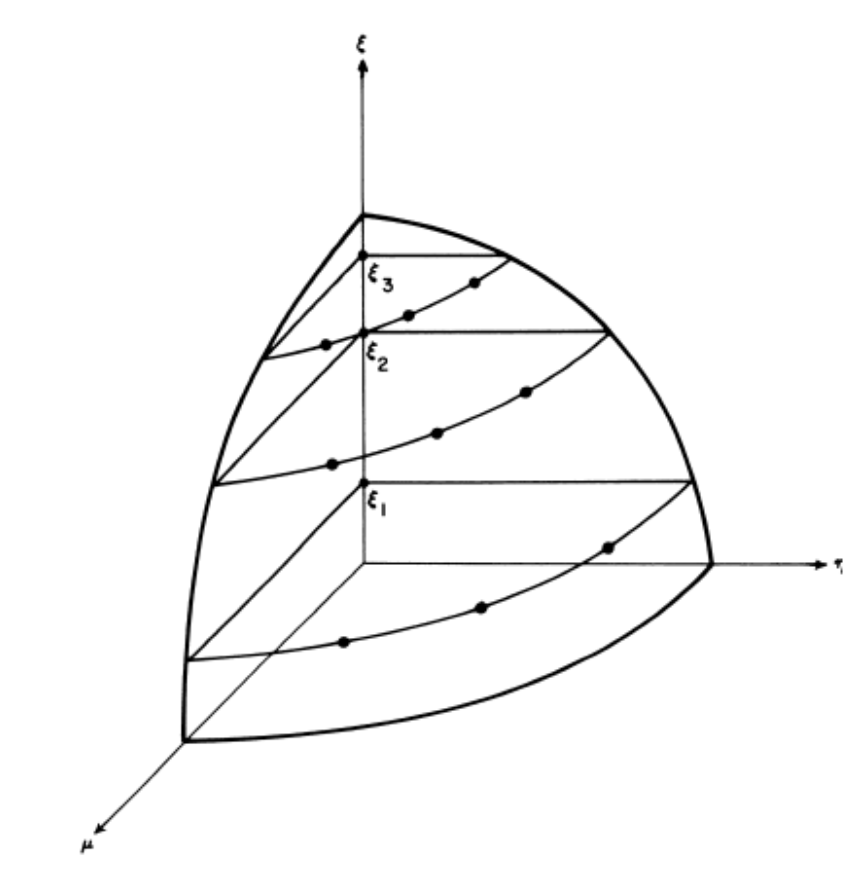
\includegraphics[width=.5\textwidth]{fig/SNPoints.png}
    \caption{Equally-Weighted Gauss-Chebyshev Quadrature Points \cite{Lathrop1965}}
    \label{fig:SN}
\end{figure}
%
Angular discretization of Eqn.~\eqref{eq:transport} is handled via the discrete ordinates ($S_N$) method, a finite-element collocation method \cite{Lathrop1965}. The $S_N$ method uses a quadrature rule, evaluating the equation at number of discrete angles or ``ordinates" and uses corresponding weights to perform a sum that results in integration over the unit sphere. 
For a set of $N$ ordinates with weights $w_n$, a function $f$ integrated over angle as
%
\begin{equation}

\int \hat{\Omega} f(\hat{\Omega}) d \hat{\Omega} = \sum\limits_{\mrm=1}^{M} w_\mrm f_\mrm.    

\end{equation}

I use a Gauss-Chebyshev angular quadrature set, which can be thought of as a product set, combining a one-dimensional Gaussian Quadrature along the polar angles and an equally-weighted Chebyshev quadrature along the azimuthal angles \cite{jarrel-thesis}. This can be seen in Figure~\ref{fig:SN}. 

The steady-state, one-group $S_N$ transport equation is given as follows,

 \begin{equation}
  \vec{\Omega}_n \cdot \nabla \psi_n \left(\vec{r}\right)+ \Sigma_{\mm{t}}\left(\vec{r}\right)\psi_n = \frac{1}{4 \pi} \Sigma_{\mm{s}}\left(\vec{r}\right) \phi\left(\vec{r}\right) + \frac{1}{4 \pi} Q\left(\vec{r}\right)\:,
  \label{eq:transport-angular}
 \end{equation}
where $n$ is the angular index and $\phi = \sum\limits_{n=1}^N \omega_n \psi_n$.


\subsection{Energy Discretization}
In the treatment of energy, the full energy spectrum is divided into several energy groups. By convention, the highest energy group is given the index, 1, with the index number going up until it reaches the lowest energy group, $G$. In expanding to multiple energy groups, scattering from one group, $\rg'$ to another, $\rg$, denoted as $\rg' \rightarrow \rg $ must be taken into account. 

The energy discretized, steady-state, transport equation is
%
 \begin{equation}
  \vec{\Omega} \cdot \nabla \psi_\rg \left(\vec{r}\right)+ \Sigma_{\mm{t}, \rg}\left(\vec{r}\right)\psi_\rg = \frac{1}{4 \pi} \sum\limits_{\rg'=1}^{G}\Sigma_{\mm{s}, \rg' \rightarrow \rg}\left(\vec{r}\right) \phi_{\rg'}\left(\vec{r}\right) + \frac{1}{4 \pi} Q_\rg\:.
  \label{eq:transport-energy}
 \end{equation}


\subsection{Spatial Discretization}
In this work, I choose to discretize in two dimensions, assuming uniformity in the third; however, all formulations could be extended to be truly 3D. Spatial discretization methods for the transport equation are usually performed using commonly-known differential equation discretization techniques such as the finite difference, finite volume, or finite element methods. In this work we, discretize using the finite element method on triangular elements (described in detail in Appendix \ref{sec:spatial}); however, TG-NDA can be used with any spatial discretization. I give the weak forms of NDA and SAAF. Their full derivations can be seen in Appendix \ref{sec:spatial}. 


\subsubsection{Weak Form of Multigroup NDA}

Given a function space $W_\mathcal{D}$, for all $\psi^*$ in $W_\mathcal{D}$, Find $\psi_{\rg} \in W_\mathcal{D}$ such that
%
\begin{equation}
 \begin{split}
  \left(D_\rg \nabla \psi_\rg^{k+1/2}, \nabla \psi^*\right)_\mathcal{D} + \left(\vec{\bf{D}}_\rg \psi_\rg^{k+1/2} , \nabla \psi^*\right)_\mathcal{D} +  \left(\Sigma_{r,\rg} \varphi_{\rg}^{k+1/2}, \psi^*\right)_\mathcal{D} &=  \\
   \left(\sum\limits_{\substack{\rg'=1}}^\mm{g-1} \Sigma_{\mm{s},\rg' \to\rg}\psi_{\rg}^{k+1/2}, \psi^*\right)_\mathcal{D} + \left(\sum\limits_{\substack{\rg'=\rg+1}}^\mm{G} \Sigma_{\mm{s},\rg' \to\rg}\psi_{\rg}^{k}, \psi^*\right)_\mathcal{D} 
  &+ \left(Q_{\rg}, \psi^*_\rg\right)_\mathcal{D} \:.
 \end{split}
 \label{k1/2}
\end{equation}
%
where the parentheses represent the inner product integrated over a domain $\mathcal{D}$ for a given direction.

\subsubsection{Weak Form of Multigroup SAAF}
Using the boundary condition treatment given in \cite{zheng-thesis}, gives the following weak form:
% Correct this part
Given a function space $W_\mathcal{D}$, for all $\psi^*_{\rg}$ in $W_\mathcal{D}$, Find $\psi_{\rg} \in W_\mathcal{D}$ such that,

\begin{equation}
\begin{split}

        \left ( \vec{\Omega}\frac{1}{\sigma_{t, \rg}}\vec{\Omega}\cdot \vec{\nabla}\psi_\rg, \vec{\nabla}\psi* \right)_\mathcal{D} -     \left < \hat{n} \cdot \hat{\Omega}\psi_\rg, \psi^* \right>_{\hat{n} \cdot \hat{\Omega} < 0, \Gamma} &+ \left ( \sigma_{t, \rg} \psi_\rg, \psi* \right )_\mathcal{D} = \\
        \left ( q_\rg, \psi* \right)_\mathcal{D} + \left ( \vec{\Omega} \frac{q_\rg}{\sigma_{t, \rg}}, \vec{\nabla}\psi* \right)_\mathcal{D} &- \left < \hat{n} \cdot {\Omega} \psi^{inc}, \psi^* \right>_{\hat{n}, \hat{\Omega} <0, \Gamma} 
    \end{split}
\end{equation}

where $q = \int_{4\pi}(\Sigma_{s, \rg \rightarrow \rg'}\phi_\rg + Q)$. 
\

\section{Previous Work}

Nonlinear Diffusion Acceleration, also known as coarse-mesh finite difference, was developed to accelerate the resolution of scattering inside of a given energy group \cite{Knoll2011} \cite{park-nda}. It has been very successful in improving run times in problems of interest and has been adopted in widely used codes such as Rattlesnake \cite{Wang2013, Schunert2017, morel-holo}. NDA pairs the lower order diffusion equation with a correction calculated using a higher order equation to maintain the higher-order transport accuracy. 

Several higher order equations have been used with NDA \cite{morel-holo, Wang2013}. In this work, I use the Self Adjoint Angular Flux equation \cite{saaf}. SAAF is a formulation that pairs well with finite element discretization, as together they produce a symmetric positive definite matrix that allow the use of linear solvers such as the conjugate gradient method \cite{Shewchuck1994}.

NDA has proven itself to be very successful when addressing the convergence within an energy group, however it does not affect the convergence of multigroup solvers. One of the most commonly used multigroup solvers, Gauss-Seidel, can converge arbitrarily slowly in problems with upscattering and little leakage or absorption. Separately, methods have been developed to accelerate the convergence of Gauss-Seidel, but to our knowledge they have not yet been tried in conjunction with NDA. 

Adams and Morel developed an upscatter acceleration scheme known as the Two-Grid method. An estimation of the error at each Gauss-Seidel iteration is calculated using a collapsed in energy, one-group diffusion equation and energy eigenvector of the Gauss-Seidel iteration matrix. These spatial and energy components make up the correction term to the scalar flux at each group, which is applied at each iteration. In one dimensional calculations, Adams and Morel have demonstrated their method to be very efficient for thermal upscattering problems \cite{morel-upscat}.

Inspired by their method, I develop a two-grid scheme for the NDA equations. The derivation is presented in the next section. 